\chapter{Theory}\label{theory} 

Chapter~\ref{introduction} introduced the concept of software paradigms, how
they arose and how, while they can calculate the same things, might lead to
different software quality. Historically and today OOP is been the most popular
language for the commercial software industry. Java is an OOP language that is,
in February 2019, the most popular language in the software industry. It is also
a multi-paradigm language, since it combines OOP with procedural programming. In
this study, when we say OOP we also imply that it is procedural from now on.
Languages that are functional, like Haskell and F\#, are used less
frequently.~\cite{tiobe} However functional concepts have become more popular in
multi-paradigm languages like Javascript. For example React, based on Functional
Reactive Programming~\cite{reactisfrp}, has gained a lot of
popularity.~\cite{popularityreact} 

Exact definitions exist of OOP but not for Functional programming. Both stated
goal is creating maintainable programs.  The way OOP makes maintainable
software is by emphasising encapsulation of state into \textit{objects} and
message passing. Functional programs emphasise moving state to the edges of the
program, making the core logic of the program pure and using immutable data
(defined in Section~\ref{functionalprogramming}). Immutable data is data whose
state can not change once initialized. This is explained further in
Section~\ref{functionalprogramming} and Section~\ref{oop}. To prevent defects,
tests need to be written to check that the behavior works as expected, thus
testability is of concern when creating maintainable software.

While paradigms define how we build our applications, we still need design
patterns for structuring the source code. A design pattern is a template for the
developer when structuring their code to solve certain problems. For instance,
without design patterns, one can couple dependencies with logic which affects
maintainability. Coupling logic and dependencies causes problems if we later
want to change the dependency since that means we also have to change the logic.
This study will present the patterns for OOP and functional programming in their
respective section. 

\section{Characteristics of Functional Programming}\label{functionalprogramming}

 While different definitions exist of what Functional programming means, we
 define functional programming as a paradigm that uses of pure functions,
 decoupling state from logic, using trait-based polymorphism and
 immutable data.

\begin{description}
\item[ Purity ]

When a function is pure it means that calling a function with the same arguments
        will always return the same value and that it does not mutate any value.
        For example if you have $f(x) = 2\cdot x$, then $f(2)$ will always
        return $4$. It follows then that an impure functions is either dependant
        on some state or mutates state in some way. For example, given $g(x) =
        currenttime \cdot x$, $g(5)$ will yield a different value depending on
        what time it is called. This makes it dependant on some state of the
        world. Or given $x=0$, $h()=x+1$. Then $h()$ will yield $x=1$ and $(h
        \circ h)()$ will yield $x=2$, making it impure.~\cite{wikipedia_pure}

	\item[ Trait-based polymorphism ]

		In OOP we inherit classes that contain methods and
attributes.~\cite{Gamma:1995:DPE:186897} For functional programs, we instead
define classes that describe the actions that are possible. For example, a
class \texttt{Equality} could contain a function \texttt{isEqual} that checks
if two data types are equal. Then any data type that implements the interface
Equality, for example lists or binary trees, would be able to use the function
isEqual.  This is known as type-classes in
Haskell\footnote{\url{www.learnyouahaskell.com/types-and-typeclasses}}, mixins
in Javascript\footnote{\url{www.typescriptlang.org/docs/handbook/mixins.html}}
or traits in Scala\footnote{\url{https://docs.scala-lang.org/tour/traits.html}}.

\item[ Immutable data by deafult ]

Immutable data is data that after initialization can not change. This means if
we initialize a record, \texttt{abc = \{a: 1, b: 2, c: 3\}} then \texttt{abc.a
= 4} is an illegal operation. Immutable data, along with purity, ensures that
no data can be mutated unless it is specifically created as mutable data.

\item[Decoupling state from logic]

Even if functional programs emphasise purity applications still need to deal
        with state somehow. For example a server would need to interact with a
        database. Functional programs solve this by separating pure functions
        and effectful functions. Effects are observable interactions with the
        environment, such as database access or printing a message.  While
        various strategies exist, like Functional Reactive
        Programming\footnote{Read more:
        \url{en.wikipedia.org/wiki/Functional_reactive_programming}},
        Dialogs\footnote{Read more:
        \url{stackoverflow.com/questions/17002119/haskell-pre-monadic-i-o}} or
        uniqueness types\footnote{Read more:
        \url{https://en.wikipedia.org/wiki/Clean_(programming_language)}}, the
        one used in Haskell, the language used in this thesis to construct the
        programs, is the IO monad. For the uninitiated, one can think of Monads
        as a way to note which functions are pure and which are effectful and
        managing the way they intermingle. It also allows us to handle errors
        and state.\footnote{This is simplified as Monads are notoriously
        difficult to explain.}. 

A strategy to further separate state and logic, one can construct a
        three-layered architecture, called the three layer Haskell cake. Here,
        the strategy is that one implements simple effectful functions,
        containing no logic as a base layer. Then on a second layer one
        implements an interface that implements a pure solution and one
        effectful solution. Then on the third layer one implements the logic of
        the program in pure code. The way the second layer is implemented is
        explained further in Section~\ref{interpreterpattern}. 
\end{description}

So while no exact definition of Functional programming exist, we here define it
as making functions pure and inheritance being based around functionality rather
than attributes.

\subsection{Sum types and product types}\label{types}

A type is in Haskell a \textit{set} of possible values that a given data can
have. This can be $int$, $char$ and custom defined types. A \textit{sum type} or
\textit{union type} is a type which is the sum of types, meaning that it can be
one of those it's given types. For example the type \texttt{type IntChar = Int |
Char} is either an Int or a Char. It can also be used to create enums such as
\texttt{type Color = Red | Green | Blue}, meaning that a value of type Color is
either red, green or blue. A product type is a type which is the product of
types, for example \texttt{type User = User Name Email}.  Informally, a product
type can be likened to a record in Javascript. A sum type can be used to model
data which may or may not have a value, by introducing the Maybe type:
\texttt{type Maybe value = Just value | Nothing}. This allows us to model
computations that might fail. For example given $sqrt(x) = \sqrt{x},\,
x\in \mathbb{Z}$ then $sqrt(-1)$ is undefined and would cause Haskell to crash.
Instead by introducing a function \texttt{safeSqrt x = if x > 0 then Just (sqrt
x) else Nothing} the program can force the developer to handle the special case
of negative numbers. 

\subsection{Brief introduction to Monads for side effects}\label{monads}

Monads\footnote{\url{en.wikipedia.org/wiki/Monad_(functional_programming)}} are
a way to sequence computations that might fail while automating away boilerplate
code. Figure~\ref{monadclass} shows how Monads are implemented as a typeclass in
Haskell. It implements the function \texttt{return}, the function bind
\texttt{(>>=)}, the function sequence \texttt{(>>)} which is bind whilst
ignoring the prior argument and \texttt{fail} which handles crashes.

\begin{figure}[H]
    \begin{lstlisting}
        class Monad m where  
            return :: a -> m a  
            (>>=) :: m a -> (a -> m b) -> m b  
            (>>) :: m a -> m b -> m b  
            fail :: String -> m a  
            fail msg = error msg 
    \end{lstlisting}
    \caption{Monad type class in Haskell.}
    \label{monadclass}
\end{figure}

Informally if this does not make sense, think of Monads as a design pattern that
allows us to sequence different computations. Without them the developer would
have to explicitly check if a computation has failed. For example, given the
function $unsafeSqrtLog = sqrt\,\circ\,log$, then $unsafeSqrtLog(-1)$ would throw an
error since $log$ and $sqrt$ are undefined for $-1$.  Section~\ref{types} showed
how the \texttt{Maybe value} type could be used to create a safe computation
\texttt{safeSqrt}. However to sequence that computation with a function
\texttt{safeLog}, the user would have to manually check that \texttt{safeSqrt}
returned a value \texttt{Just result} and not \texttt{Nothing}. Monads allows 
sequencing these computations without explicitly writing this check, so
composing \texttt{safeSqrt} and \texttt{safeLog} using bind becomes
\texttt{safeSqrtLog n = safeSqrt n >>= safeLog}. The same idea applies for
effectful computations such as fetching data from a database.

\subsection{Interpreter pattern for testability}\label{interpreterpattern}

The beginning of this chapter briefly mentioned that design patterns are
important to create maintainable software.  In this study a design pattern
called the Interpreter pattern will be used to structure functional programs. An
interpreter is something which interprets input of some format, modifies it and
transforms it into some output.  Informally, we can think of interpreter pattern
as a way to create smaller composable compilers that when added together make
one big application. A compiler is a program that takes some input, interprets
the input and then does some output. A server, for example, would take some
request, interpret that request and then turn it into a response. The server
could integrate itself with the database, which would take some query, interpret
that query and then return an object.~\cite{interpreterpattern}

To implement this pattern in Haskell we create an Abstract Syntax Tree (AST),
using a union type\footnote{\url{https://en.wikipedia.org/wiki/Union_type}}, of
the program that contains all the available commands that the program is capable
of doing. See Figure~\ref{freeunion} for an example of a to-do list AST. Once we
have the AST we can encode the logic of the program as instructions. Then the
final step is to implement an interpreter for the program that evaluates those
commands. So if we have the commands in Figure~\ref{freeunion}, we implement a
function \texttt{eval} that takes a command and computes some effectful code.
The command \texttt{Add Item (Item -> next)} could, for example, be executed as
add an Item to a database.

\begin{figure}[H]
    \begin{lstlisting}
       data TodoList next
            = Add Item (Item -> next)
            | Mark Item next
            | Remove Item next
            | End --^ Terminates the program
    \end{lstlisting}
    \caption{AST for a to-do-list. We can derive a functor instances
    from ASTs for deriving Free instances.~\cite{commentarycompiler}}
    \label{freeunion}
\end{figure}


Hiding the implementation behind an AST allows us to separate effectful code
(like output a string or send a http request) with the logical instructions.
This simplifies our testing, since we can hide the environment (for example
database) behind an interface that we can swap out for testing. So we can
implement two interpreter functions, one for our real environment and one for
testing. 

\subsection{Using MTL for the interpreter pattern}\label{mtl}

To implement the interpreter pattern described in
Section~\ref{interpreterpattern} one can use MTL. Using MTL means that we can
substitute our dependencies by using a type class so that we have one pure and
one effectful instance. Then afterwards the pure instance can be used for
testing. 

For example, if one wants to implement an authentication system for a server
where the tokens expire within one week then one could do it as shown in
Figure~\ref{tokennaive}. Figure~\ref{tokennaive} is hard to test as it couples
effectful code with pure code. The function \texttt{token} depends on the
current time and that makes unit testing more difficult.

\begin{figure}[H]
    \begin{lstlisting}

    addWeek :: POSIXTime -> POSIXTime
    addWeek currentTime =
        currentTime + oneWeek
        where
            oneWeek = 604800000

    token :: Key User -> IO (Maybe WebToken)
    token user =
        do  currentTime <- Time.Posix.getPOSIXTime
            let expirationDate = addWeek currentTime
            let maybeToken = encode $ Token user expirationDate
            return maybeToken
    \end{lstlisting}
    \caption{Example of a function that, given the ID of a user, generates a
    unique token that can be used for authentication.}
    \label{tokennaive}
\end{figure}

Instead, by using the MTL technique, one decouples the effectful code from it's
dependencies. In Figure~\ref{tokennaive} the effectful code is the function
\texttt{Time.Posix.getPOSIXTime}, which fetches the current time. So the type
class will be a class \texttt{MonadTime} that contains one method
\texttt{getTime}. By abstracting away the effectful code it becomes trivial to
implement a pure and effectful instance. This is done in
Figure~\ref{tokencorrect}. 

\begin{figure}[H]
    \begin{lstlisting}
    class MonadTime m where
        getTime :: m POSIXTime

    instance MonadTime IO where
        getTime = Time.Posix.getPOSIXTime

    instance MonadTime ((->) POSIXTime) where
        -- Allows us to call functions with the constraint MonadTime
        -- with an extra argument containing a mock value.
        getTime = id

    addWeek :: POSIXTime -> POSIXTime
    addWeek currentTime =
        currentTime + oneWeek
        where
            oneWeek = 604800000

    token :: MonadTime m => Key User -> m (Maybe WebToken)
    token user =
        do  currentTime <- getTime
            let expirationDate = addWeek currentTime
            let maybeToken = encode $ Token user expirationDate
            return maybeToken
    \end{lstlisting}
    \caption{An implementation of the token generation following MTL and
    interpreter pattern.}
    \label{tokencorrect}
\end{figure}

With the implementation in Figure~\ref{tokencorrect}, testing the function
\texttt{token} becomes trivial with the instance \texttt{MonadTime ((->)
POSIXTime)} as it allows one to substitute \texttt{getTime} with any value. Thus
we separate effectful code from logic and mocking becomes trivial.


\section{SOLID principles}\label{oop}


In Chapter\label{introduction} and earlier in this chapter we established the
basics of OOP. The way to design a OOP system is left to it's user. If the
design of a system is done poorly, it can lead to rotten design. Martin Robert,
a software engineer, claims that there are four big indicators of rotten design.


\begin{description}

\item[ Rigidity ] Rigidity is the tendency for software to be difficult to
change. This makes it difficult to change non-critical parts of the software and
what can seem like a quick change takes a long time.

\item[ Fragility ] Fragility is when the software tends to break when doing
simple changes. It makes the software difficult to maintain, with each fix
introducing new errors.

\item[ Immobility ] Immobility is when it is impossible to reuse software from
other projects in the new project. So engineers discover that, even though they
need the same module that was in another project, too much work is required to
decouple and separate the desirable parts.

\item[ Viscosity ] 

Viscosity comes in two forms: the viscosity of the environment and the viscosity
of the design. When the engineer makes changes they are often met with multiple
solutions. Some that preserve the design and some that are ``hacks''. So the
engineer can easily do the wrong thing. When the compile times are long the
engineers will attempt to make changes that do not cause long compile times.
This leads to viscosity in the environment.
\end{description}

To avoid creating rotten designs, Martin Robert proposes the SOLID guideline.
SOLID mnemonic for five design principles to make software more maintainable,
flexible and understandable. The SOLID guideline is

\begin{description}
    \item [Single responsibility principle] Here, responsibility means ``reason
        to change''. Modules and classes should have one reason to change and no
        more.
    \item [Open/Closed principle] States we should write our modules to be
        extended without modification of the original source code.
    \item [Liskov substitution principle] Given a base class and an derived
        class derive, the user of a base class should be able to use the derived
        class and the program should function properly.
    \item [Interface segregation principle] No client should be forced to depend
        on methods it does not use. The general idea is that you want to split
        big interfaces to smaller, specific ones.
    \item [Dependency inversion principle] A strategy to avoid making our source
        code dependent on specific implementations is by using this principle.
        This allows us, if we depend on one third-party module, to swap that
        module for another one should we need to. This can be done by creating
        an abstract interface and then instance that interface with a class that
        calls the third-party operations.~\cite{martinrobert}
\end{description}

Using a SOLID architecture helps make programs that are not as dependent on the
environments, making them easier to test (as we can swap the production
environment to a test environment). When investigating the testability, it is
important that to look at programs that are written in such a way that all parts
are easy to test. Thus choosing a SOLID architecture for OOP based programs will
allow making more testable software.

\section{Measuring testability and complexity}\label{measuretestability}

The previous sections defined the programming paradigms and how to write
software in a testable and maintainable manner. Since the aim of the study is to
find which of the two paradigms allows us to write the most maintainable
software. looking at the \textit{Cyclomatic complexity} of software it is
possible to find out the amount of tests needed to test every possible outcome
of the software. It follows then that if one of the paradigms have a lower
complexity, it would require less tests. If less tests need to be written, it is
sound to assume that the amount of lines of code (LOC) needed for the software
would be lower. Lower LOC correlates with less defects in
software.~\cite{defectloc} 

Looking at the testability of code for maintenance is not enough. While
testability is an important metric, it can also be important to look at other
factors like how cognitive complexity affects the maintenance. For instance, a
program written in the language Whitespace, an esoteric language consisting only
of whitespace\footnote{Description of Whitespace:
\url{https://en.wikipedia.org/wiki/Whitespace_(programming_language)}}, could
have a low LOC and cyclomatic complexity. But for humans knowing only the
English language, a text consisting of whitespace would be illegible. By using a
framework called Cognitive dimensions to do a qualitative evaluation of
software one can qualitatively the structural software quality. This is described
further in Section~\ref{cognitivedimensions}.


\subsection{Measuring testability: Cyclomatic Complexity}\label{cyclomaticcomplexity}

Cyclomatic complexity is a complexity measure that allows us to measure the
amount of paths through a program. The Cyclomatic complexity number is an upper
bound for the number of test cases required for full branch coverage of the
code. 

\theoremstyle{definition}
\begin{definition}
The cyclomatic number $v(G)$ of a graph G with $n$ vertices, $e$ edges and $p$
connected components is $v(G) = e - n + p$.
\end{definition}

\begin{theorem}
In a strongly connected graph $G$, the cyclomatic number is equal to the
maximum number of linearly independent circuits.~\cite{McCabe}
\end{theorem}

Informally, cyclomatic complexity is a way to measure the amount tests a program
needs to reach full branch coverage by constructing a graph that branches out
based on the control flow. For example, given \texttt{f(bool) = if bool then
``hello''; else ``hola''} the function \texttt{f} will either evaluate to
``hello'' or ``hola''. To get full branch coverage for \texttt{f} two tests are
needed. The cyclomatic complexity therefore becomes 2. The nodes of a cyclomatic
graph represents processing tasks and edges represent control flow between
the nodes. 

Given the code found in example figure~\ref{c1excode}. To calculate the
complexity of this function, first construct a graph as seen in
figure~\ref{fig:c1exgraph}. From the graph we find $n=4, e=5, p=2\Rightarrow
v(G)=e-n+p=5-4+2=3$ is the cyclomatic number.

\begin{figure}[H]
    \begin{lstlisting}
        void foo(void)
        {
          if (a)
            if (b) 
              x=1;
          else
              x=2;
         }
    \end{lstlisting}
    \caption{Multi if function foo.}
    \label{c1excode}
\end{figure}


\begin{figure}[H]
    \centering
    \begin{tikzpicture}
        \tikzset{vertex/.style = {shape=circle,draw,minimum size=2.5em}};
        \tikzset{edge/.style = {->,> = latex'}};
        \node[vertex] (a) at (2,8) {\texttt{if (a)}};
        \node[vertex] (b) at (0,6) {\texttt{if (b)}};
        \node[vertex] (c) at (4,6) {\texttt{x=2}};
        \node[vertex] (d) at (2,4) {\texttt{end}};
        \draw[edge] (a)  to (b);
        \draw[edge] (a)  to (c);
        \draw[edge] (b)  to (c);
        \draw[edge] (b)  to (d);
        \draw[edge] (c)  to (d);
    \end{tikzpicture}
    \caption{Cyclomatic complexity graph for Figure~\ref{c1excode}}
    \label{fig:c1exgraph}
\end{figure}

\subsection{Cyclomatic Complexity in Functional
Programming}

The definition of cyclomatic complexity in Section~\ref{cyclomaticcomplexity} is
not ideal for functional programming. Cyclomatic complexity is calculated by
creating graphs based on control flow operations such as while loops and if
statements. In functional programming everything is a function, thus the
cyclomatic complexity will always tend to 0 using this definition. So we define
a different method of calculating the cyclomatic complexity for functional
programs. 

\theoremstyle{definition} 
    \begin{definition} 
    The cyclomatic complexity number, in functional programming, is equal to
    1 plus the sum of the left hand side, called LHS, plus the sum of the
    right hand side, called RHS. RHS is the sum of the number of guards,
    logical operators, filters in a list comprehension and the pattern
    complexity in a list comprehension. LHS is equal to the pattern
    complexity.  The pattern complexity is equal to the number of
    identifiers in the pattern, minus the number of unique identifiers in
    the pattern plus the number of arguments that are not identifiers. In
    summary:

    \begin{lstlisting}
    Cyclomatic complexity = 1 + LHS + RHS

    LHS = Pattern complexity 

    Pattern complexity   
        = Pattern identifiers 
        - Unique pattern identifiers 
        + Number of arguments that are non identifiers

    RHS = Number of guards 
        + Number of Logical operators 
        + Number of filters in list comprehension 
        + Pattern complexity in list comprehension
    \end{lstlisting}
\end{definition}

Instead of cyclomatic graphs in functional programs one constructs flowgraphs,
such as the one seen in Figure~\ref{fig:cyclomaticfunctional}, to model the
functions.

\begin{figure}[H]
    \begin{lstlisting}
    split :: (a -> Bool) -> [a] -> ([a], [a])
    split onCondition [] = ([], [])
    split onCondition (x:xs) =
        let 
            (ys, zs) = split onCondition xs
        in 
            if (onCondition x) then 
                (x:ys, zs)
            else 
                (ys, x:zs)
    \end{lstlisting}
    \caption{Recursively split a list into two based on a given condition in
    Haskell. For example \texttt{split (>3) [1,2,3,4,5] =
    ([4,5],[1,2,3])}.}
    \label{split}
\end{figure}

In Haskell $(x:xs)$ denotes an item $x$ at head of a list of items $xs$. Given
the Haskell code in Figure~\ref{split}. To calculate LHS we find two
pattern identifiers which are $onCondition$ and $(x:xs)$. there is one unique
pattern identifiers which is $(x:xs)$. There is also one non identifier
which is $[]$. There is also one guard, an if statement, and no
list comprehensions on RHS. Thus the cyclomatic complexity is $1+(2-1+1)+1=4$.

In this method to calculate cyclomatic complexity, do not count the $otherwise$
and $else$ clauses.~\cite{bergklaas}


\begin{figure}[H]
    \centering
    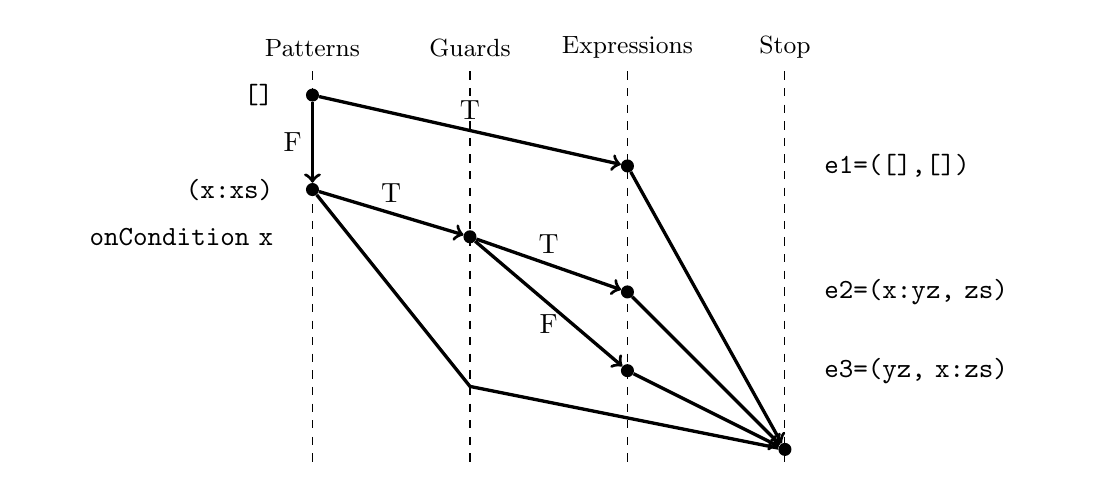
\begin{tikzpicture}
        \tikzset{vertex/.style = {shape=circle,fill=black,scale=0.5}};
        \draw[dashed] (0,0) -- (0,-5) (2,0) -- (2,-5) (4, 0) -- (4, -5) (6, 0)
        -- (6, -5);
        \node at (0,.3) {\small{Patterns}};
        \node at (2,.3) {\small{Guards}};
        \node at (4,.3) {\small{Expressions}};
        \node at (6,.3) {\small{Stop}};
        \node[vertex] (a) at (0,-0.3) {};
        \node[align=right, text width=3cm] at (-2,-0.3) {\texttt{[]}};
        \node[vertex] (b) at (4,-1.2) {};
        \draw[->, very thick] (a) to node [above] (TextNode) {T} (b) ;
        \node[vertex] (c) at (0,-1.5) {};
        \node[align=right, text width=3cm] at (-2,-1.5) {\texttt{(x:xs)}};
        \draw[->, very thick] (a) to node [left] (TextNode) {F} (c) ;
        \node[align=left, text width=3cm] at (8,-1.2) {\texttt{e1=([],[])}};
        \node[vertex] (d) at (2,-2.1) {};
        \draw[->, very thick] (c) to node [above] (TextNode) {T} (d) ;
        \node[align=right, text width=3cm] at (-2,-2.1) {\texttt{onCondition x}};
        \node[vertex] (e) at (4,-2.8) {};
        \draw[->, very thick] (d) to node [above] (TextNode) {T} (e) ;
        \node[align=left, text width=3cm] at (8,-2.8) {\texttt{e2=(x:yz, zs)}};
        \node[vertex] (f) at (4,-3.8) {};
        \draw[->, very thick] (d) to node [below] (TextNode) {F} (f) ;
        \node[align=left, text width=3cm] at (8,-3.8) {\texttt{e3=(yz, x:zs)}};
        \node[vertex] (g) at (6,-4.8) {};
        \draw[->, very thick] (e) to (g) ;
        \draw[->, very thick] (b) to (g) ;
        \draw[->, very thick] (f) to (g) ;
        \draw[very thick] (c) to (2, -4.0) to (g) ;
    \end{tikzpicture}
    \caption{Flowgraph for split function, defined in Figure~\ref{split}.}
    \label{fig:cyclomaticfunctional}
\end{figure}

Cyclomatic complexity finds how many tests are needed to get full branch
coverage of source code. A low complexity for a program means that less tests
have to be written.  Note that if a program has a low cyclomatic complexity it
does not imply that the program is easier to test. If a program is written in
such a way that it depends heavily on the environment it can also lead to
difficulty testing. So to make cyclomatic complexity a better metric this study
will use design patterns to make testable code.

\subsection{Mental complexity: Cognitive Dimensions}\label{cognitivedimensions}

Cognitive Dimensions is a framework for evaluating the usability of programming
languages and to find areas of improvements.~\cite{GREEN1996131} It allows us to
evaluate the quality of a design and explore what future improvements could be
made. As part of the Cognitive Dimensions, 14 different Cognitive Dimensions of
Notation exist. A notation depends on the specific context, in this case the
notation is the languages themselves and their architecture. The author of the
framework recommends omitting the dimensions that are not applicable to the
notation. We give a brief description of the dimensions.

\begin{description}

\item[ Viscosity ]

How much work does it take to make small changes? How easy is the code to
refactor? If small changes requires consequent adjustments then that is a
problem. As a viscous system cause a lot more work for the user and break the
line of thought.

\item[ Visibility ]

How easy is it to navigate the source code to find the parts that you want?

\item[ Hidden dependencies ]

Are there hidden dependencies in the source code. Does a change in one part of
the source code lead to unexpected consequences in another part of the code.
Every dependency that matters to the user should be accessible in both
directions. 

\item[ Role-expressiveness ]

How obvious is each sub-component of the source code to the solution as a whole?

\item[ Abstraction ]

What are the levels of abstraction in the source code? Can the details be
encapsulated?

\item[ Secondary notation ]

Are there any extra information being conveyed to the user in the source code?

\item[ Closeness of mapping ]

By looking at the source code, how close do we find it to be to the case
we are solving?

\item[ Consistency ]

Once Object-oriented procedural programming and Functional programming has been
learned. How much of the rest can the user guess successfully? 

\item[ Diffuseness or terseness ]

How much space and symbols does the source code need to produce a certain result
or express a meaning?

\item[ Hard mental operations ]

Where does the hard mental processing lie? Is it more when writing the source
code itself rather than solving the case, I.E. the semantic level? Does one
sometimes need to resort to pen and paper to keep track of what is happening?

\item[ Provisionality ]

How easy is it to get feedback of something before you have completed the entire
system?

\item[ Progressive evaluation ]

How obvious the role of each component of the source code in the solution as a
whole?

\item[ Error proneness ]

To what extent does the programming paradigm and language help minimise errors? Are
there any structures or complexities that lead to it being easier to make
errors?
\end{description}

\noindent For this study we will investigate the following dimensions: 

\begin{itemize}
    \item Diffuseness or terseness
    \item Progressive evaluation
    \item Closeness of mapping
    \item Hard Mental Operations
    \item Visibility
    \item Hidden dependencies
    \item Abstraction
    \item Error-proneness 
\end{itemize}

\noindent We omit the other dimensions as related work concluded that the other
dimensions did not bring much weight when evaluating the different
paradigms.~\cite{euguenkiss}

In summary, cognitive dimensions allow us to look at different aspects of a
programming language to evaluate how complex they are cognitively. 

